\section{Optics}

\subsection{Geometrical Optics}

\paragraph{Optical Path length}
For light to travel a distance $d$ in a material with refractive index $n$, it takes
a time $t = \frac{d}{v} = \frac{n d}{c}$. We call $D = n \cdot d$ the optical path length.

\paragraph{Fermat's Principle}
Light travelling between two points will follow a path whose optical path length is
extremal to variations in the path


\paragraph{Snell's Law}

$n_1 \sin(\theta_1) = n_2 \sin(\theta_2)$

\paragraph{Paraxial Approximation}
Only consider rays that make a small angle with respect to some optical
axis.

\paragraph{Single Surface Lens:}

\begin{enumerate}[]
    \item \fat{Radius of Convergence}:
        $\frac{1}{R} = \frac{1}{n_2 - n_1} \klammer{\frac{n_1}{d_1} - \frac{n_2}{d_2}}$
    \item \fat{Focal Length}: $f = \frac{R \cdot n_2}{n_2 - n_1}$, $\frac{n_2}{f} = \frac{n_1}{s_o} + \frac{n_2}{s_i} = \frac{n_2 - n_1}{R}$
\end{enumerate}

\paragraph{Two-Surface Lens:}

\begin{enumerate}[]
    \item \fat{Focal Length}: $\frac{n_w}{s_o} + \frac{n_w}{s_i} = (n_l - n_w) \klammer{\frac{1}{R_1} - \frac{1}{R_2}}$
        with $n_w$ the refractive index of the surrounding and $n_l$ the refractive index
        of the material of the lens. Further: $\frac{1}{f_w} = \frac{1}{s_o} + \frac{1}{s_i}
        = \klammer{\frac{n_l}{n_w} - 1} \klammer{\frac{1}{R_1} - \frac{1}{R_2}}$
    \item \fat{Thin lens formula / lensmaker's formula}: $\frac{1}{f} = \frac{1}{d_1} + \frac{1}{d_2}
        = \frac{1}{f_1} + \frac{1}{f_2}$
    \item \fat{Characteristics}: \begin{enumerate}[a)]
        \item $f>0$: converging lens (Light is bent towards the optical axis)
        \item $f<0$: diverging lens (Light is bent away from the optial axis)
        \item $d_1 = s>0$: real object, before lens
        \item $d_1 = s<0$: virtual object, after lens
        \item $d_2 = d>0$: real image, after lens
        \item $d_2 = d<0$: virtual image, before lens
    \end{enumerate}
    \item \fat{Maginfication Factor}: $M = - \frac{d_2}{d_1} = \frac{h'}{h}$ where
        $h$ is the hight of the object and $h'$ is the hight of the image. If
        $M>0$: image is upright, if $M<0$: image is inverted.
\end{enumerate}

\paragraph{Telescope} $\Delta \theta' \approx \frac{f_1}{f_2} \Delta \theta$.
Here, $\theta$: incident angle, $f_1$: focal length lens 1, $f_2$: focal length
lens 2, $\theta'$: angle after passing through two lenses.

\paragraph{Microscope} Total magnification: $M = \frac{d_1 d_2}{s_1 s_2}$.
Here, $s_1$: distance object and lens 1, $s_2$: distance image lens 1 and
lens 2, $d_1$: distance image lens 1 and lens 1, $d_2$: distance virtual image
lens 2 and lens 2. Note: $d_2$ is negative, thus the image is inverted.



\subsection{Wave Optics}

\paragraph{Maxwell's Equations and Wave Equations in vacuum}
\begin{align*}
    \vec{\nabla} \cdot \vec{E} = 0
    \hspace{5pt} , \hspace{5pt}
    \vec{\nabla} \cdot \vec{B} = 0
    \hspace{15pt} &, \hspace{15pt}
    \vec{\nabla} \times \vec{E} = - \frac{\partial \vec{B}}{\partial t}
    \hspace{5pt} , \hspace{5pt}
    \vec{\nabla} \times \vec{B} = \mu_0 \epsilon_0 \frac{\partial \vec{E}}{\partial t}
    \\
    \vec{\nabla}^2 \vec{E} = \frac{1}{c^2} \frac{\partial^2 \vec{E}}{\partial t^2}
    \hspace{5pt} &, \hspace{5pt}
    \vec{\nabla}^2 \vec{B} = \frac{1}{c^2} \frac{\partial^2 \vec{B}}{\partial t^2}
\end{align*}

\paragraph{Superposition Principle}
Every linear combination of solutions to the wave equation is again a solution
to the wave equation.

\paragraph{Huygens' Principle}
Every point on the "wavefront" of a wave acts as a secondary source of hemispherical
waves that propagate in the "forward" direction. Here, "wavefront" means surfaces
in space where the eletrical field has the same phase of oscillation.

\vspace{1\baselineskip}

Consider a source $A$ at $\vec{r}_A = (x_A , y_A , z_A)$ and a detector $B$ at
$\vec{r}_B = (x_B , y_b , z_B)$ with an aperture of cross section $a^2$ between
the two. Take $C$ a point in the apperture. Then the spatial part of the electric
field emmited from $A$ at $C$ is given by
\begin{align*}
    U \propto \frac{1}{\abs{\vec{r}_C - \vec{r}_A}} e^{i k \abs{\vec{r}_C - \vec{r}_A}}
    \hspace{5pt} , \hspace{5pt}
    \abs{\vec{r}_B - \vec{r}_C} = \sqrt{(x-x_A)^2 + (y-y_A)^2 + z_A^2}
\end{align*}
Similarly we can write the electrical field at point $B$ due to the spherical
wave at $C$. In the end, the total electric field at $B$ is given by
\begin{align*}
    U \propto \int_{-a/2}^{a/2} dx \int_{-a/2}^{a/2} dy \
    \frac{1}{\abs{\vec{r}_C - \vec{r}_A} \cdot \abs{\vec{r}_B - \vec{r}_A}}
    e^{i k \klammer{\vec{r}_C - \vec{r}_A} + \abs{\vec{r}_B - \vec{r}_A}}
\end{align*}
\begin{align*}
    \abs{\vec{r}_C - \vec{r}_A} &= \sqrt{x_A^2 + y_A^2 + z_A^2 - 2 x x_A - 2 y y_A + x^2 + y^2}
    \\
    &\approx r_A - \frac{x x_A + y y_A}{r_A} + \frac{x^2 + y^2}{2 r_A}
    \\
    &\approx r_A - \frac{x x_A + y y_A}{r_A}
\end{align*}
where $r_A = \sqrt{x_A^2 + y_A^2 + z_A^2}$ and similarly for $r_B$. The first
assumption made is $a \ll r_A , r_B$. The secons approximation of dropping the
quadratic terms and is called \fat{Fraunhofer approximation}.
\begin{align*}
    U_B \propto \int_{-a/2}^{a/2} dx \int_{-a/2}^{a/2} dy
    \frac{e^{i k (r_A + r_B)} e^{-i k (X x + Y y)}}{\klammer{r_A - \frac{x x_A - y y_A}{r_A}} \klammer{r_B - \frac{x x_B - y y_B}{r_B}}}
\end{align*}
Where $X = \frac{x_A}{r_A} + \frac{x_B}{r_B}$ and $Y = \frac{y_A}{r_A} + \frac{y_B}{r_B}$.
With third approximation, dropping the fractions in the denominator, we obtain:
\begin{align*}
    U_B &\propto \frac{e^{i k (r_A + r_B)}}{r_A r_B} \int_{-a/2}^{a/2} dx \int_{-a/2}^{a/2} dy \ e^{-i k (X x + Y y)} 
    \\
    &\propto \frac{a^2 e^{i k (r_A + r_B)}}{r_A + r_B} \text{sinc} \klammer{\frac{k X a}{2}} \text{sinc} \klammer{\frac{k Y a}{2}}
\end{align*}
With Fermat's Principle we obtain that $U$ is extremal if $X = 0$ and $Y=0$.
In general we can introduce a aperture function $t(x,y)$ so that
\begin{align*}
    U_B \propto e^{i k (r_A + r_B)} \intii dx \intii dy \ t(x,y) \ e^{-ik(X x + Y y)}
\end{align*}

\paragraph{Rayleigh Criterion}
Two objects are just resolved if the intensity maximum of one lines up with the
intensity minimum of the other. Equivalent:
\begin{align*}
    \frac{x_{A_2}}{r_{A_2}} = \sin(\theta_S) > \frac{\lambda}{a}
    \hspace{10pt} , \hspace{10pt}
    \theta_s = \sin^{-1} \klammer{\frac{\lambda}{a}}
\end{align*}
Where the index $2$ should indicate that it is the second light source, the first
one is on the optical axis. $\theta_S$ is the so called \fat{angular resolution}.


\paragraph{Abbé Limit}
In the spacial resolution of microscopes, the Abbé Limit describes the limit
at which two slits in a diffraction pattern are still distinguishable.
\begin{align*}
    d > \lambda \frac{\sqrt{s^2 + (L/2)^2}}{L}
\end{align*}
where $d$ is the distance between the two slits, $s$ is the distance between the
lense and the slits and $L$ is the diameter of the lens.

\paragraph{Numerical apperture}
$N_A = sin(\theta_{\text{lense}}) \approx \frac{w_l}{2 d_l}$
with $w_l = $ lense width and $d_l = $ distance object to lense


\subsection{Polarization}

\paragraph{Linear Polarization}
\begin{align*}
    \vec{E}(\vec{r},t) &= \klammer{E_x \hat{x} + E_y \hat{y}} \cos(kz-\omega t)
    \\
    &= E_0 \klammer{\cos(\theta) \hat{x} + \sin(\theta) \hat{y}} e^{i(kz - \omega t)}
\end{align*}

\paragraph{Elliptical and circular Polarizations}
\begin{align*}
    \vec{E}(\vec{r},t) &= E_x \hat{x} \cos(k z - \omega t) + E_y \hat{y} \cos(k z - \omega t + \phi)
    \\
    &= \klammer{E_x \hat{x} + E_y e^{i \phi} \hat{y}} e^{i (k z - \omega t)}
\end{align*}
In the case of $\phi = \pm \frac{\pi}{2}$ we have a circle. If $\phi = \frac{\pi}{2}$,
we have right circular polarization and if $\phi = - \frac{\pi}{2}$ we have left
circular polarization.

\paragraph{Birefringence}
A birefringent is a material that has different refraction indices for the $x$ and
$y$ component of an electric field.

\paragraph{Maxwell's Equations: macroscopic version}
\begin{align*}
    \vec{\nabla} \cdot \vec{D} = 0
    \hspace{5pt} , \hspace{5pt}
    \vec{\nabla} \cdot \vec{B} = 0
    \hspace{5pt} , \hspace{5pt}
    \vec{\nabla} \times \vec{E} = - \frac{\partial \vec{D}}{\partial t}
    \hspace{5pt} , \hspace{5pt}
    \vec{\nabla} \times \vec{H} = \frac{\partial D}{\partial t}
\end{align*}
$\vec{B} = \mu_0 \mu_r \vec{H}$, $\vec{D} = \epsilon_0 \epsilon_r \vec{E}$,
speed of light in a material with refraction index $n$: $v = \frac{c}{n}$,
$n = \sqrt{\mu_r \epsilon_r}$, $\vec{k} \times \vec{B} = \omega \vec{B}$,
$B = \frac{k}{\omega} E = \frac{n k_0}{\omega} E = \frac{n}{c} E$.

\paragraph{Refraction and Reflection at a surface}

\begin{figure}[h]
    \centering
    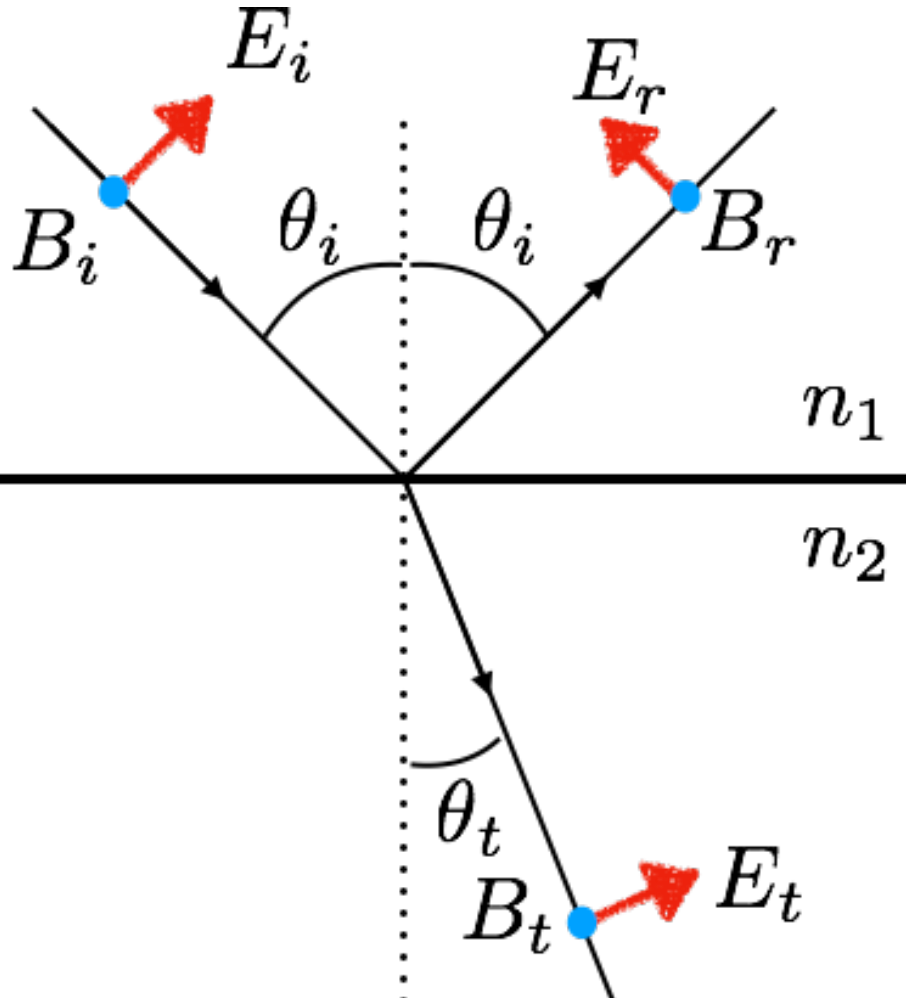
\includegraphics[width=0.2\textwidth]{Figures/p-polarization.png}
    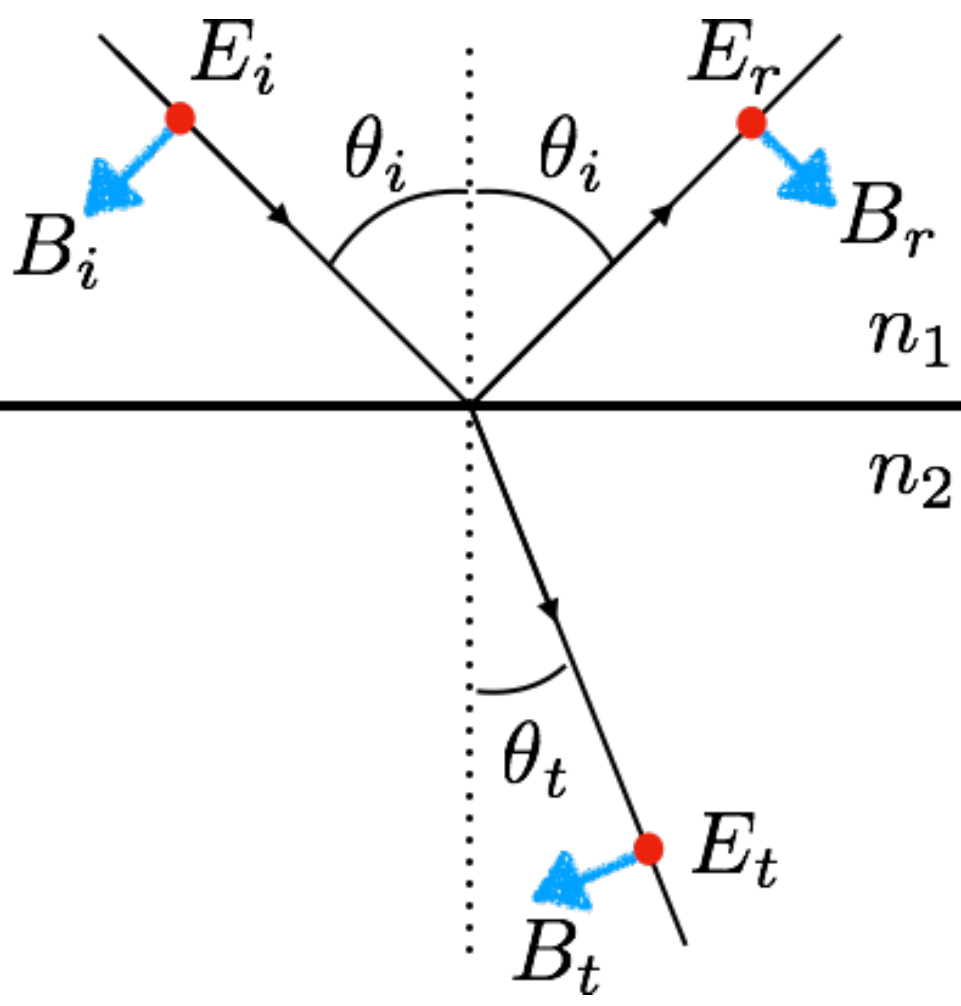
\includegraphics[width=0.2\textwidth]{Figures/s-polarization.png}
    \caption{Left: p-polarization, Right: s-polarization}
\end{figure}

Boundry conditions for amplitudes of plane waves across a planar interface:
\begin{align*}
    B_{\perp 1} = B_{\perp 2}
    \hspace{5pt} , \hspace{5pt}
    D_{\perp 1} = D_{\perp 2}
    \hspace{5pt} , \hspace{5pt}
    H_{\parallel 1} = H_{\parallel 2}
    \hspace{5pt} , \hspace{5pt}
    E_{\parallel 1} = E_{\parallel 2}
\end{align*}

With this we have: $E_i \cos(\theta_i) - E_r \cos(\theta_i) = E_t \cos(\theta_t)$
and $n_1 E_i + n_1 E_r = n_2 E_t$.

\subparagraph{Fresnel Equations}
\begin{enumerate}[]
    \item For p-polarization:
        \begin{align*}
            t_p &= \frac{E_t}{E_i} = \frac{2 n_1 \cos(\theta_i)}{n_2 \cos(\theta_i) + n_1 \cos(\theta_t)}
            \\
            r_p &= \frac{E_r}{E_i} = \frac{E_r}{E_i} = \frac{n_2 \cos(\theta_i) - n_1 \cos(\theta_t)}{n_2 \cos(\theta_i) + n_1 \cos(\theta_t)}
                = \frac{\tan(\theta_i - \theta_t)}{\tan(\theta_i + \theta_t)}
        \end{align*}
    \item For s-polarization:
        \begin{align*}
            t_s &= \frac{E_t}{E_i} = \frac{2 n_1 \cos(\theta_i)}{n_1 \cos(\theta_i) + n_2 \cos(\theta_t)}
            \\
            r_s &= \frac{E_r}{E_i} = \frac{n_1 \cos(\theta_i) - n_2 \cos(\theta_t)}{n_1 \cos(\theta_i) + n_2 \cos(\theta_t)}
        \end{align*}
\end{enumerate}


\paragraph{Brewster's Angle}

$r_p = 0 \Leftrightarrow \theta_i + \theta_t = \frac{\pi}{2}$. This special value
of $\theta_i$ is called Brewster's angle, labeled $\theta_B = \arctan(n_2/n_1)$.
For light waves incident at an angle of $\theta_B$, no p-polarized light can be
reflected. For s-polarized light, there is no incidence angle where there is no
zero reflectivity.


\subsection{Spectroscopy}

\paragraph{Grating Spectrometer}
Phase difference between the light reflecting off of two neighboring stips:
\begin{align*}
    \phi(\lambda) = k d \klammer{\sin(\theta_i) - \sin(\theta_j)}
    \hspace{10pt} , \ k = \frac{2 \pi}{\lambda}
\end{align*}
Contribution from $N$ strips:
\begin{align*}
    U &\propto \sum_{n=0}^{N-1} e^{i n \phi} = \frac{1 - e^{i N \phi}}{1 - e^{i \phi}}
    = e^{i(N-1)\phi/2} \frac{\sin\klammer{N \phi / 2}}{\sin(\phi/2)}
    \\
    I &\propto \abs{U}^2 \propto \frac{\sin^2 \klammer{N \phi / 2}}{\sin^2(\phi/2)}
\end{align*}
Maxima at $\phi/2 = m \pi$ with $m \in \Z$. Maximal value: $N^2$. Yields:
\begin{align*}
    \sin(\theta_i) - \sin(\theta_j) = \frac{2 \pi m}{d k} = \frac{m \lambda}{d}
\end{align*}
$m$ is the \fat{order of the maximum}. Condition for Minima:
\begin{align*}
    \frac{\phi_2}{2} = \klammer{m + \frac{1}{N}} \pi
\end{align*}
Combinint conditions:
\begin{align*}
    \phi_2 - \phi_1 &= \frac{2 \pi}{N}
    \\
    k_2 - k_1 &= \frac{2 \pi}{N d \klammer{\sin(\theta_i) - \sin(\theta_j)}}
    \\
    \Delta \nu &= \frac{c}{N d \klammer{\sin(\theta_i) - \sin(\theta_j)}}
\end{align*}


\paragraph{Interferometry}
Consider Michelson inferometer. Beamsplitter devides input beams evenly into two
parts of equal amplitude and phase and does the inverse of this on recombination.
Electric field on detector:
\begin{align*}
    U \propto \frac{1}{2} U_0 e^{2 i k d_1} + \frac{1}{2} U_0 e^{2 i k d_2}
    = \frac{U_0}{2} e^{2 i k d_1} \klammer{1+e^{2 i k x}}
\end{align*}
where $U_0$ is the input amplitude, $d_1$ and $d_2$ are the optical path lengths
and $x = d_2 - d_1$. With this:
\begin{align*}
    I \propto \frac{\abs{U_0}^2}{4} \klammer{2 + 2 \cos(2 k x)}
    \propto \frac{I_0}{2} \klammer{1+\cos(4 \pi x / \lambda)}
\end{align*}

The \fat{spectral density} $S(\nu)$ of a light source:
$S(\nu) d \nu$ is the power emitted by the light source between frequencies
$\nu$ and $\nu + d \nu$.
\begin{align*}
    I &\propto \int_0^\infty S(\nu) \klammer{1+\cos(4 \pi x / \lambda)} \ d \nu
    \\
    &\propto \int_0^\infty S(\nu) \ d \nu + \int_0^\infty S(\nu) \cos(4 \pi \nu x / s) \ d \nu
    \\
    &\propto \int_0^\infty S(\nu) \ d \nu + \frac{1}{2} \intii S(\abs{\nu}) e^{i 4 \pi \nu x / c} \ d \nu
\end{align*}
\begin{align*}
    S(\nu) &\propto \int_0^\infty \klammer{2 I(x) - I_0} \cos(4 \pi \nu x / c) \ d x
    \\
    &\sim \int_0^{x_{\text{max}}} \klammer{2 I(x) - I_0} \cos(4 \pi \nu x / c) \ d x
    \\
    &\sim \int_0^{x_{\text{max}}} \cos (4 \pi x \nu_0 / c) \cos(4 \pi x \nu / c) \ dx
    \\
    &\sim \text{sinc} \klammer{\frac{2 \pi (\nu - \nu_0) x_{\text{max}}}{c}}
        + \text{sinc} \klammer{\frac{2 \pi (\nu + \nu_0) x_{\text{max}}}{c}}
\end{align*}
This peaks at $\nu = \pm \nu_0$. Zeros closest to the maximum at $+\nu_0$ are at
\begin{align*}
    \nu - \nu_0 = \pm \frac{c}{2 x_{\text{max}}}
\end{align*}
Thus, according to Rayleigh criterion our spectrometer resolution is
\begin{align*}
    \frac{\Delta \nu}{\nu_0} = \frac{\lambda}{2 x_{\text{max}}}
    \hspace{10pt} \text{ or } \hspace{10pt}
    \delta \nu = \frac{c}{2 x_{\text{max}}}
\end{align*}

\paragraph{Fabry-Perot etalon}
Incomming light source: $A_0 e^{i(k x - \omega t)}$, $t$: transmission coefficient,
$r$: reflection coefficient. Transmitted field: $A_0 \cdot t$, reflected field:
$A_0 \cdot r \cdot e^{i \phi_r}$. Total field amplitude from all the paths:
\begin{align*}
    A &= A_0 t^2 e^{i k d} \sum_{n=0}^\infty r^{2n} e^{i n \phi}
    = A_0 t^2 e^{i k d} \cdot \frac{1}{1 - r^2 e^{i \phi}}
    \\
    \eta = \frac{\abs{A}^2}{\abs{A_0}^2} &= \frac{t^4}{\klammer{1 - r^2 e^{i \phi}} \klammer{1 - r^2 e^{-i \phi}}}
        = \frac{t^4}{1 + r^4 - 2 r^2 \cos(\phi)} 
    \\
    &= \frac{\klammer{1-R}^2}{(1-R)^2 + 2 R (1-\cos(\phi))}
        = \frac{1}{1 + \frac{4 R}{(1-R)^2} \sin^2 \klammer{\frac{\phi}{2}}}
    \\
    \eta = \frac{I_o}{I_i} &= \frac{1}{1+ \frac{4 R}{(1-R)^2} \sin^2 \klammer{2 \pi d / \lambda + \phi_r}}
\end{align*}
with $T = t^2$, $R = r^2$ and $t^2 + r^2 = 1$. $R$ is the reflectivity of the
mirror, $d$ the distance between the mirrors, and $\lambda$ is the wavelength
of the light, and $\phi_r$ is the phase picked up by the light when it reflects off
a mirror.
Wavelength resolution $\delta \nu$:
\begin{align*}
    \frac{d \lambda}{d \nu} = \frac{d}{d \nu} \klammer{\frac{c}{\nu}} = - \frac{c}{\nu^2}
    \hspace{10pt} \Rightarrow \hspace{10pt}
    \delta \lambda = \frac{c}{\nu^2} \delta \nu
\end{align*}

